\section{Experiment: Position-Length}

This is the one where we estimate two selected bars compared to the longest one - very similar to the previous one but, not yet done. We basically test divided versus grouped barchart and we estimate one relation between two marked quanitities: what percent the smaller is of the larger.

There are five types: type 1-3 this is a position judgement along a common scale. (btw all classifiers seem to do that extremely well in the elementary tasks so we assume this will work well here too). Types 4-5 are length judgements and we know that the classifiers struggle with that quite a bit.

The setup from Cleveland McGill is first a classification task: which one is smaller? and then a regression task: how much smaller. So we have to see how to encode this.


\subsection{Hypotheses}

We proposed two hypotheses entering the elementary perceptual task experiment:

\begin{itemize}
	\item \textbf{H3.1} \textbf{Grouped bar charts are better computational perceivable than divided bar charts.} A grouped bar chart involves judging a position while a divided bar chart most likely (if not the bottom is looked at) requires length judgements. Classifiers are better at judging position than at judging length so grouped bar charts are easier to grasp in terms of computational perception.
	\item \textbf{H3.2} \textbf{not yet} Any ideas?
\end{itemize}


%\begin{figure*}[t]
%	  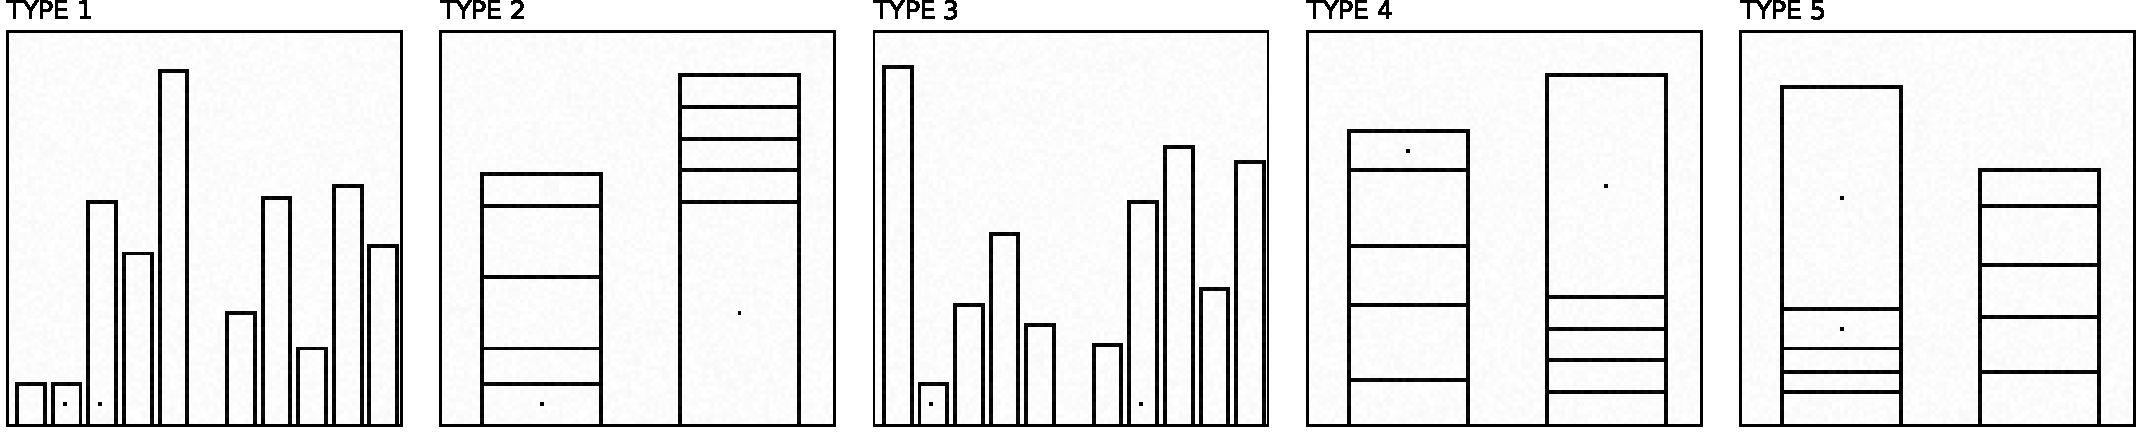
\includegraphics[width=\linewidth]{figure4_overview.pdf}
%	  
%  \caption{\textbf{Position-Length Experiment.} (Not yet) Rasterized versions of the graphs of Cleveland and McGill's position-length experiment. The perceptual task involves comparing. the two dot-marked quantities across five different visual encodings of either grouped or divided bar charts. We evaluate which type of bar chart performs better with our neural networks as a combined classification and regression problem. The first task is to select which of the marked quantities is smaller (classification) and the second task is to specify how much smaller it is (regression).}
%	\label{fig:position_length_experiment}
%\end{figure*}
\begin{table}[h]
\centering
\caption{\textbf{Position-Length Experiment.} Rasterized versions of the graphs of Cleveland and McGill's position-length experiment. The perceptual task involves comparing the two dot-marked quantities across five different visual encodings of either grouped or divided bar charts. We evaluate which type of bar chart performs better with our neural networks. The two marked values are chosen from a set of ten pairs which defines the dual regression task. Since the other 8 values are chosen randomly, the parameter space for images of this experiment is massive.}
\resizebox{\linewidth}{!}{
\begin{tabular}{lllr}
	\toprule
	\multicolumn{2}{l}{~} & ~ & Permutations\\
	\midrule
	\raisebox{-.85\height}{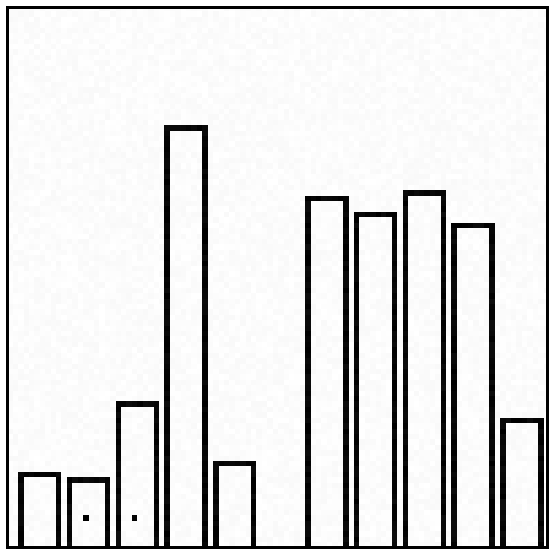
\includegraphics[width=.5in]{figure4_type_1.pdf}} & \makecell[tl]{Type 1: \emph{Grouped Bar Chart}\\~~~Perceptual Task: \emph{Position}\\~ \\~ \\} &~& \makecell[tr]{~\\ $9.20E+16$}\\

	\midrule
	\raisebox{-.85\height}{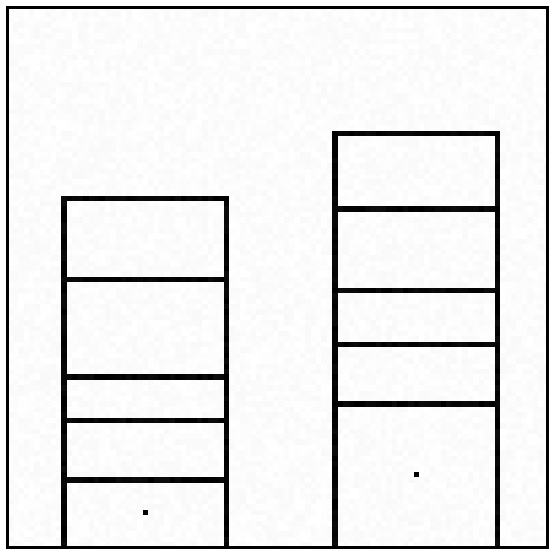
\includegraphics[width=.5in]{figure4_type_2.pdf}} & \makecell[tl]{Type 2: \emph{Divided Bar Chart}\\~~~Perceptual Task: \emph{Position}\\~ \\~ \\} &~& \makecell[tr]{~\\ $9.20E+16$}\\
	
	\midrule
	\raisebox{-.85\height}{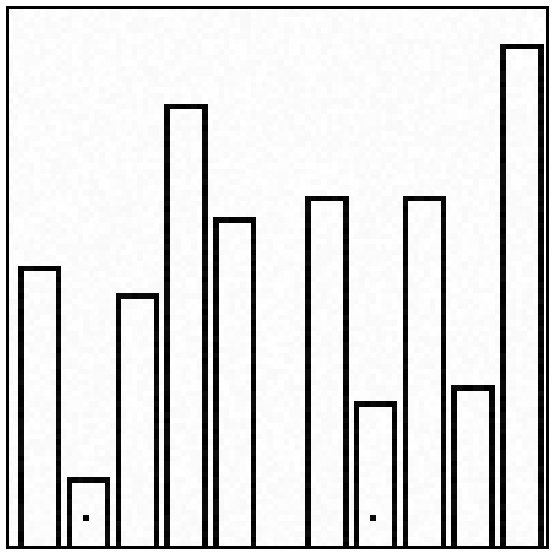
\includegraphics[width=.5in]{figure4_type_3.pdf}} & \makecell[tl]{Type 3: \emph{Grouped Bar Chart}\\~~~Perceptual Task: \emph{Position}\\~ \\~ \\} &~& \makecell[tr]{~\\ $9.20E+16$}\\
	
	\midrule
	\raisebox{-.85\height}{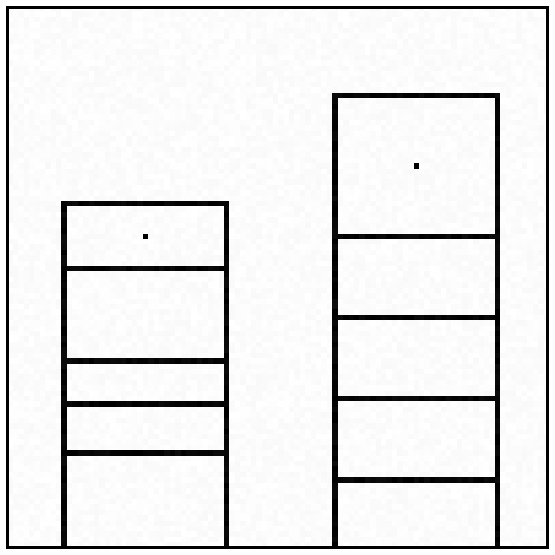
\includegraphics[width=.5in]{figure4_type_4.pdf}} & \makecell[tl]{Type 4: \emph{Divided Bar Chart}\\~~~Perceptual Task: \emph{Length}\\~ \\~ \\} &~& \makecell[tr]{~\\ $9.20E+16$}\\
	
	\midrule
	\raisebox{-.85\height}{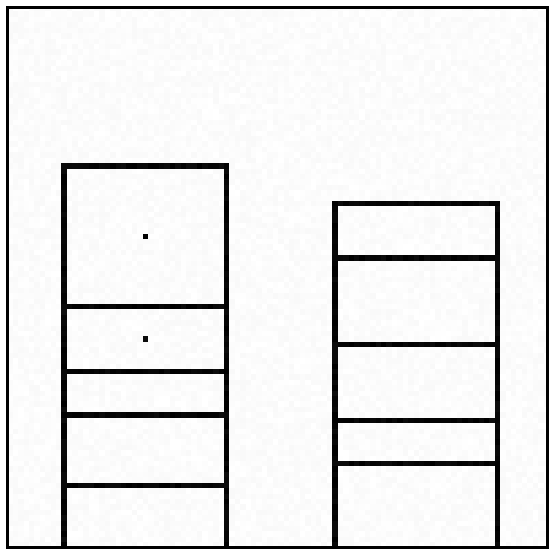
\includegraphics[width=.5in]{figure4_type_5.pdf}} & \makecell[tl]{Type 5: \emph{Divided Bar Chart}\\~~~Perceptual Task: \emph{Length}\\~ \\~ \\} &~& \makecell[tr]{~\\ $9.20E+16$}\\

	\bottomrule
\end{tabular}
}
\label{tab:pos_length_parameters}
\end{table}

\subsection{Discussion}

JT: Look at the relative difficulty of the tasks. In Cleveland and McGill, types 1-5 were post-ordered by their log error such that type 1 was easiest and type 5 was hardest. Is this still the case with our CNNs?

\subsection{Results}


\begin{figure}[t]
	\centering
	  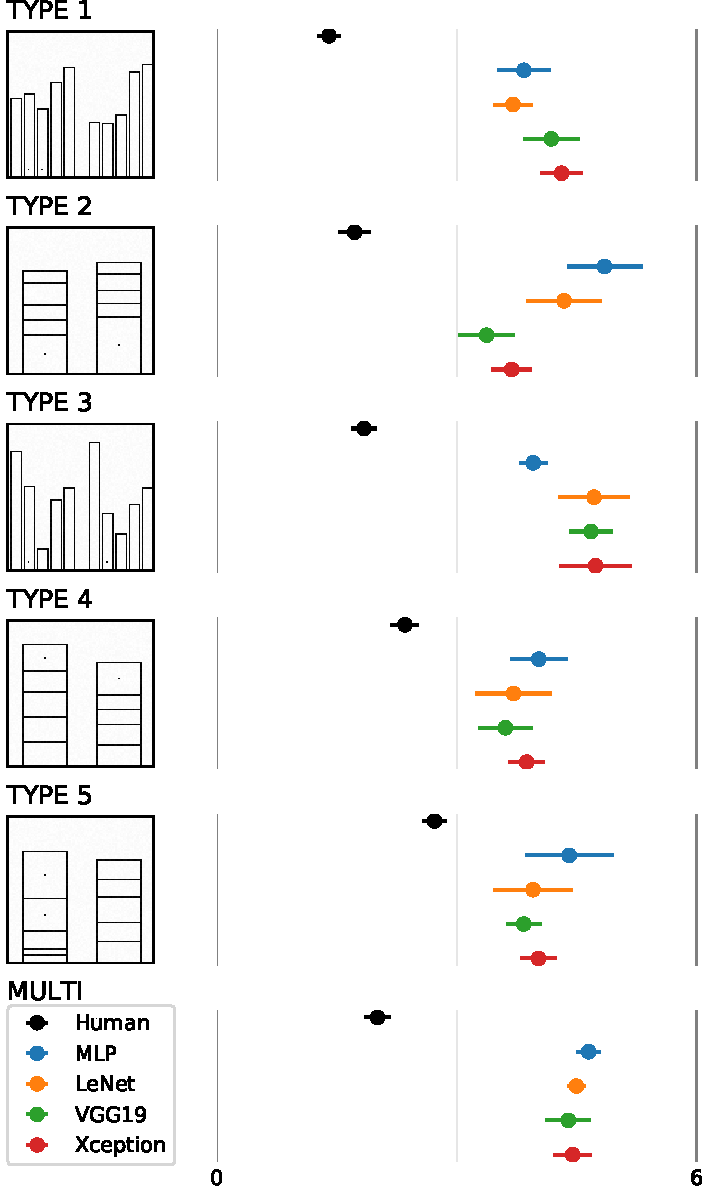
\includegraphics[width=.8\linewidth]{figure4_mlae_with_multi_and_humans.pdf}
  \caption{\textbf{Computational results of the Position-Length experiment.} Log absolute error means and 95\% confidence intervals for the \emph{position-length experiment} as described by Cleveland and McGill~\cite{cleveland_mcgill}. We test the performance of a Multi-layer Perceptron (MLP), the LeNet Convolutional Neural Network, as well as feature generation using the VGG19 and Xception networks trained on ImageNet.}
	\label{fig:figure4_mlae}
\end{figure}
